% !TeX program = pdfLaTeX
\documentclass[12pt]{article}
\usepackage{amsmath}
\usepackage{graphicx,psfrag,epsf}
\usepackage{enumerate}
\usepackage{natbib}
\usepackage{textcomp}
\usepackage[hyphens]{url} % not crucial - just used below for the URL
\usepackage{hyperref}

%\pdfminorversion=4
% NOTE: To produce blinded version, replace "0" with "1" below.
\newcommand{\blind}{0}

% DON'T change margins - should be 1 inch all around.
\addtolength{\oddsidemargin}{-.5in}%
\addtolength{\evensidemargin}{-.5in}%
\addtolength{\textwidth}{1in}%
\addtolength{\textheight}{1.3in}%
\addtolength{\topmargin}{-.8in}%

%% load any required packages here



% tightlist command for lists without linebreak
\providecommand{\tightlist}{%
  \setlength{\itemsep}{0pt}\setlength{\parskip}{0pt}}



\usepackage[dvipsnames]{xcolor} % colors
\newcommand{\aak}[1]{{\textcolor{blue}{#1}}}
\newcommand{\svp}[1]{{\textcolor{RedOrange}{#1}}}
\newcommand{\yg}[1]{{\textcolor{Green}{#1}}}
\usepackage[capitalise]{cleveref}
\newcommand\pcref[1]{(\cref{#1})}
\usepackage{algorithm,algpseudocode,booktabs}
\usepackage{booktabs}
\usepackage{longtable}
\usepackage{array}
\usepackage{multirow}
\usepackage{wrapfig}
\usepackage{float}
\usepackage{colortbl}
\usepackage{pdflscape}
\usepackage{tabu}
\usepackage{threeparttable}
\usepackage{threeparttablex}
\usepackage[normalem]{ulem}
\usepackage{makecell}
\usepackage{xcolor}

\begin{document}


\def\spacingset#1{\renewcommand{\baselinestretch}%
{#1}\small\normalsize} \spacingset{1}


%%%%%%%%%%%%%%%%%%%%%%%%%%%%%%%%%%%%%%%%%%%%%%%%%%%%%%%%%%%%%%%%%%%%%%%%%%%%%%

\if0\blind
{
  \title{\bf A Spatio-Temporal Model for Arctic Sea Ice}

  \author{
        Alison Kleffner 1 \\
    Department of Statistics, University of Nebraska - Lincoln\\
     and \\     Susan VanderPlas 2 \\
    Department of Statistics, University of Nebraska - Lincoln\\
     and \\     Yawen Guan 3 \\
    Department of Statistics, University of Nebraska - Lincoln\\
      }
  \maketitle
} \fi

\if1\blind
{
  \bigskip
  \bigskip
  \bigskip
  \begin{center}
    {\LARGE\bf A Spatio-Temporal Model for Arctic Sea Ice}
  \end{center}
  \medskip
} \fi

\bigskip
\begin{abstract}
Arctic Sea Ice is a barrier between the warm air of the ocean and the
atmosphere, thus playing an important role in the climate. When narrow
linear cracks (leads) form in the sea ice, the heat from the ocean is
released into the atmosphere. To estimate where cracks may form, motion
data from the RADARSAT Geophysical Processing System (RGPS) is analyzed.
RGPS provides a set of trajectories of points on the ice sheet to trace
the displacement of sea ice, however, chunks of data are missing due to
the data collection method by satellite. We propose a spatio-temporal
clustering and interpolation method that estimates where a crack may
form and allows us to infer missing observations. Features based on the
sea ice displacement are created for k-means clustering by creating a
bounding box around each trajectory, resulting in trajectories being
assigned a cluster. A crack is considered to have formed on the boundary
between different clusters. Within the clusters, a spatio-temporal
interpolation model using a Gaussian Process is used to infer missing
locations. Our clustering approach is compared to ice lead detection
methods, and cross-validation is used to assess our interpolation
method.
\end{abstract}

\noindent%
{\it Keywords:} spatial clustering, non-stationary, Gaussian process
\vfill

\newpage
\spacingset{1.45} % DON'T change the spacing!

\hypertarget{introduction}{%
\section{Introduction}\label{introduction}}

Sea ice in the Arctic Ocean that acts as an insulator between the warm
ocean and the cooler atmosphere \citep{peterson_evaluating_2011}.
However, sea ice is constantly changing and moving due to dynamic
processes, including wind and ocean current, which causes leads in the
ice to form \citetext{\citealp{peterson_evaluating_2011}; \citealp[
]{hoffman_detection_2019}; \citealp{hutter_leads_2019}}. When a lead
forms in the sea ice it provides a significant source of heat and
moisture into the atmosphere, which reduces the overall sea ice
concentration and warms the regional atmospheric boundary layer
\citep[\citet{reiser_new_2020}]{key_detectability_1993}. Additionally,
the formation of leads also has an affect on atmosphere and ocean
chemical exchanges, which include carbon dioxide and mercury
\citep{hoffman_detection_2019}. Thus, the state of the sea ice,
including lead characteristics, provides important information for
weather prediction, climate models, and ocean models
\citep{reiser_new_2020}. When leads form, this may be an indicator of
climate change, and may also be a driver of climate change due to the
release of warmer air \citep{peterson_evaluating_2011}.

Current methods to determine the location of leads generally either
involve the use of thermal infrared satellite data or the calculation of
ice deformation using movement. Thermal methods tend to use thermal
channels from the Advanced Very High Resolution Radiometer (AVHRR), as
the surface temperatures between a lead and the surrounding sea ice are
different \citep{key_detectability_1993}. Using thermal channels from
the AVHRR is highly dependent on clear skies as clouds can also give a
higher temperature and may be mistaken for a lead. Methods have been
suggested to reduce the impact of clouds.
\citet{willmes_pan-arctic_2015} uses only clear sky pixels from the
Moderate Resolution Imagery Spectroradtiometer (MODIS). However, MODIS
has issues with low and thin clouds. Hence, a fuzzy cloud artifact
filter was used to remove any remaining clouds, but there is a trade-off
between parameterization and error rates. \citet{rohrs_algorithm_2012}
suggested using passive microwave data as clouds are transparent at
microwave wavelengths. However, microwave data lacks wide spatial
coverage and has coarse resolution making detecting narrow leads
impossible \citep{hoffman_detection_2019}.

Deformation methods to locate leads is determined by the motion of sea
ice. These methods use NASA's RADARSTAT Geophysical Processing System
(RGPS), which uses synthetic aperture radar (SAR) images to track the
trajectory of points on Arctic sea ice. To track trajectories, points
are initially assigned to a vertex of a grid cell on an ice sheet, which
is tracked over time using the SAR satellite images. Then the
deformation of the ice is calculated within each grid cell, where areas
of high deformation may be denoted as leads
\citep{peterson_evaluating_2011}. These methods can provide additional
information about a lead, such as size and deformation. However,
satellite images only pass the same area typically every three to six
days, thus we do not have a complete set of space-time observations to
calculate deformation. Additionally, the error in the deformation
calculations may be strongly underestimated as the grid cells may become
distorted due to movement, which affects deformation calculations
\citep{bouillon_producing_2015}.

When working with dynamic data, like the ocean surface, the
spatio-temporal dynamics need to be reconstructed in order to
interpolate. Satellite-derived data used to monitor dynamic items can
have large missing data rates either due to the sampling rate of
atmospheric conditions \citep{fablet_data-driven_2017}. Thus, if we want
to have complete gridded data, interpolation is necessary. In optimal
interpolation, the model of the covariance function of the
spatio-temporal field-dynamics is used. The interpolated field is a
result of a linear combination of the observations, assuming stationary
\citep{fablet_data-drive_2017, ouala_neural_2018}. Additionally, due to
large amounts of data being collected, data driven methods have become
popular. For example, data assimilation involves the construction of a
dynamical systems made using the data
\citep{li_variational_2015, fablet_data-drive_2017, ouala_neural_2018}.

Often when working with data relating to the environment, a simple
global mean and covariance function is inaccurate as the relationships
between variables may change over space. Hence, when developing a
non-stationary spatio-temporal model, the mean and parameter function
should have different parameters depending on the region. Therefore, a
non-stationary model can be developed, either through a Gaussian Process
or Bayesian Hierarchical framework, where the covariance function
parameters varies by different regions
\citep{guinness_nonstationary_2013, SALVANA2020100411}.

Our proposed method for lead detection also uses the movement of the ice
sheet. However, ice sheet movement is not consistent, as the underlying
process will cause the ice sheet to move differently depending on the
location resulting in leads \citep{peterson_evaluating_2011}. Thus, we
aim to determine lead location by finding clusters of similar movement,
where the boundaries between the clusters are the location of cracks.
Additionally, using the information gained from clustering, we developed
a non-stationary spatio-temporal interpolation method to estimate
missing points along a trajectory. Within a cluster, all trajectories
move in a similar fashion, so would expect a missing point to move
similarly to observed points in the cluster. Hence, we can then create a
completely gridded dataset that can be used to calculate deformation.

\hypertarget{data}{%
\section{Data}\label{data}}

Data on the movement of the ice sheet comes from NASA's RADARSTAT
Geophysical Processing System (RGPS). RGPS data is useful as it is
independent of cloud coverage and has broad spatial coverage.
Trajectories of around 30,000 points are tracked by RGPS using
sequential synthetic aperture radar (SAR) images on the Arctic sea ice
\citep{lindsay_radarsat_2003}. To track these points, an initial grid is
created at the start of the study period where each cell dimension is 10
km on a side \citep{kwok_seasonal_2002}. The vertex of each cell is
assigned an identifier \(g\). In each SAR image, the points is found
again using area-based and feature-based tracking
\citep{peterson_evaluating_2011}. The trajectories of each identifier
\(g\) form a set of all trajectories
\(\mathcal{G} =\left\{g_1,...,g_n\right\}\), where
\(g_j = \left\{s_{jt}: t \in \mathcal{T}_j\right\}\). The location of
\(g_j\) is represented as \(s_{jt} = (x_{jt}, y_{jt})\) or a set of
latitudes and longitudes. Most \(g_j\) are tracked in three day
intervals, however sampling can be irregular
\citep{peterson_evaluating_2011}. Thus,
\(\mathcal{T}_j \subset \left\{1,...,T\right\}\), which is a collection
of time points where identifier \(g_j\) is observed. We focus on the
Beaufort region, which has n = 8811 and \(T\)=22.

\begin{figure}[tbp]

{\centering 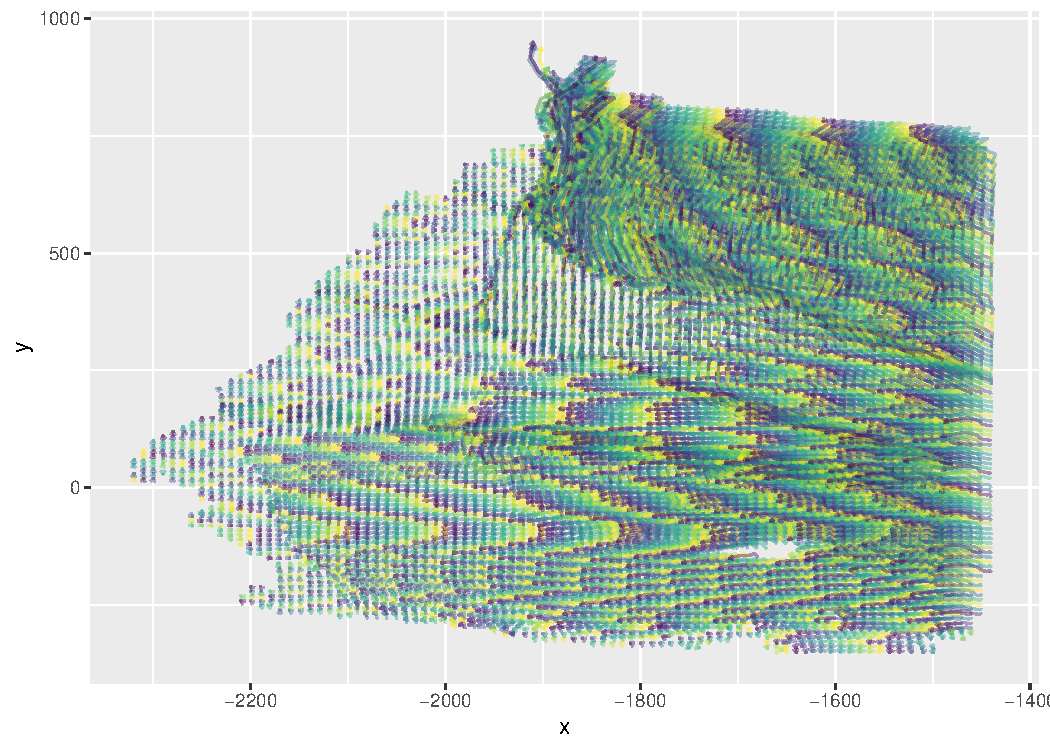
\includegraphics[width=\linewidth,]{spatio-temporal-model-arctic-sea-ice_files/figure-latex/trajectories-1} 

}

\caption{Plot of only known locations of each $g_j$, represented by a line, to show movement. An arrow is given to indicate direction of movement. The color of each $g_j$ does not have special meaning, they are just used to distinguish individual trajectories.}\label{fig:trajectories}
\end{figure}

Since we want to detect cracks only using movement data, it is first
important to visualize the movement. Thus, a plot of the trajectory of
each \(g_j\) is found in \cref{fig:trajectories}. This figure shows that
groups of trajectories appear to move with similar patterns. For
instance, at the top of \cref{fig:trajectories}, a group of trajectories
are traveling upwards, while in the middle a group is traveling from
right to left. Visualizing the movement led to the idea of clustering
similar trajectories, since the similar movement happens in continguous
patches. The movement of each trajectory can be summarized by a bounding
box. This allows for the creation of features that can be used in a
clustering algorithm, and it circumnavigates the missing data issue.
After the bounding box features are created, the trajectories are
grouped with other that have similar features. Leads are considered to
be location on the boundary between groups, as these groups are moving
differently.

\hypertarget{methods}{%
\section{Methods}\label{methods}}

\hypertarget{spatio-temporal-clustering-bounding-box}{%
\subsection{Spatio-Temporal Clustering: Bounding
Box}\label{spatio-temporal-clustering-bounding-box}}

\begin{figure}[tbp]

{\centering 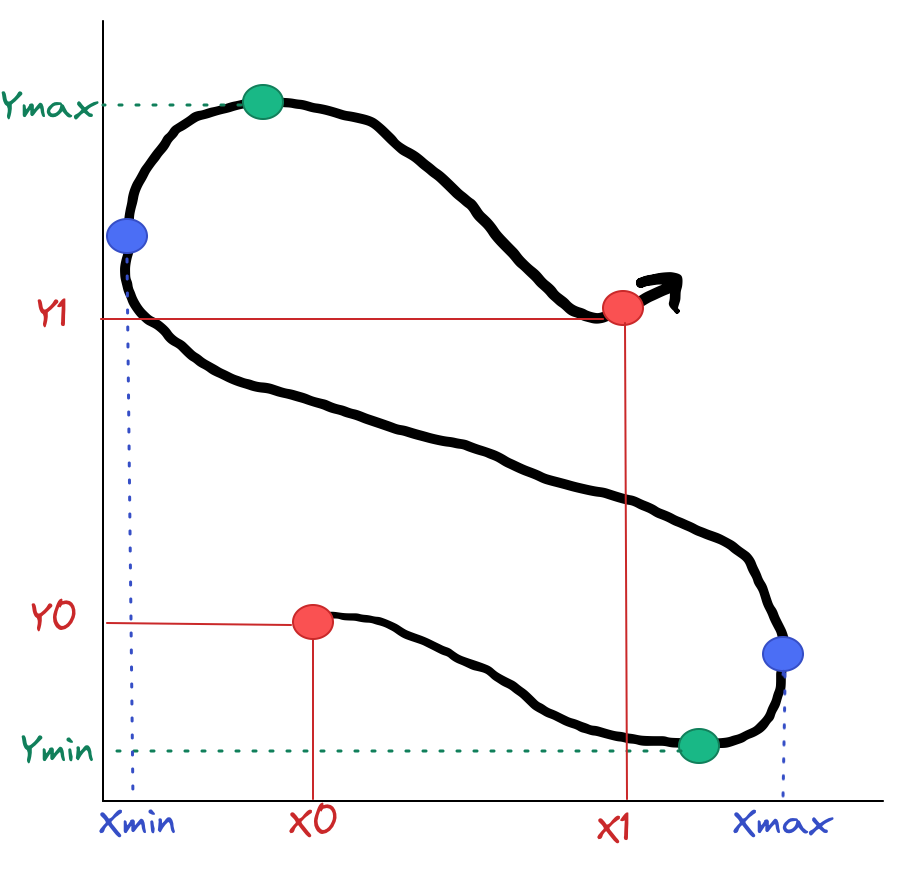
\includegraphics[width=0.5\linewidth,]{images/bounding-box} 

}

\caption[Bounding Example]{Picture of points used to calculate features of our Bounding Box}\label{fig:bb-pic}
\end{figure}

\hypertarget{bounding-box-features}{%
\subsubsection{Bounding Box Features}\label{bounding-box-features}}

The bounding box that is created around each trajectory is used to
derive features that represent it's movement. Features includes the
length traveled between the minimum and maximum location of a coordinate
(\(x_{max} - x_{min}\) and \(y_{max} - y_{min}\)), representing the
total distance traveled. However, the maximum and minimum locations may
not always correspond to the first and last day of the time frame.
Hence, the difference in each coordinate (\(x_{1} - x_{0}\) and
\(y_{1} - y_{0}\)) from the latest observation to the earliest
observation in the time frame was also found. The change from latest to
the earliest observation is then used to calculate the angle of change
to find the direction of movement of the trajectory. Further, since the
focus is on the cluster boundaries, we must ensure the clusters are
contiguous, meaning clusters are not co-located across multiple
geographic locations. To ensure some geographic continuity, we also
include the average coordinate values for each trajectory.

A bounding box can be created around a whole trajectory, or for smaller
sub-trajectories. Sub-trajectories may provide more information while
ensuring adequate data is available for the clustering process. A
balance between ensuring data completeness and capturing sufficient
movement is essential. If creating a bounding box for a sub-trajectory,
for instance by week, the features from the previous week may be
included as inputs into the clustering algorithm. This is done to ensure
some consistency between consecutive time frames, as previous movement
may impact current movement. After all of the different features are
calculated, the values are then standardized to give each feature
similar weight in the clustering process.

\hypertarget{k-means}{%
\subsubsection{K-Means}\label{k-means}}

We partitioned \(n\) trajectories into \(k\) clusters using k-means
clustering, with \(k\) being a pre-specified number. The goal of this
method is to minimize the squared Euclidean distance between the
features of an observation and the centroid vector of a cluster, which
is made up of the average features of the cluster members
\citep{steinley_kmeans_2006}. This method requires each observation to
be in a cluster, which is beneficial as we want to know what group each
trajectory is more similar to. However, a drawback of k-means is that
the number of clusters must be known and specified prior to clustering.
We determine the number of clusters using the silhouette statistic,
which compares within cluster distances to between cluster distances
\citep{kodinariya_2013}. Ice movement is a dynamic process, so if
clustering sub-trajectories, like weeks, then we would expect that each
week to have a different number of clusters. Thus, when clusters were
created by week, we calculated the silhouette statistic separtely for
each week.

\hypertarget{spatio-temporal-interpolation}{%
\subsection{Spatio-Temporal
Interpolation}\label{spatio-temporal-interpolation}}

\hypertarget{finding-spatio-temporal-neighbors}{%
\subsubsection{Finding Spatio-Temporal
Neighbors}\label{finding-spatio-temporal-neighbors}}

\begin{figure}[tbp]

{\centering 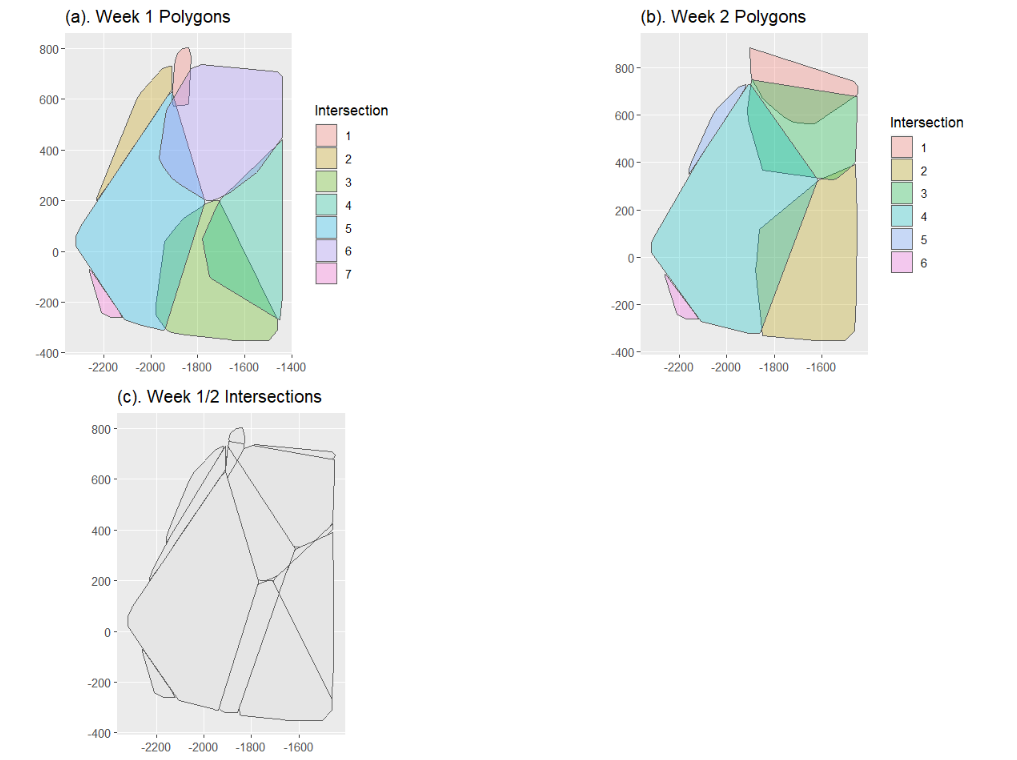
\includegraphics[width=0.7\linewidth,]{images/int-one} 

}

\caption{(a). Polygons of week 1 clusters (b). Polygons of week 2 clusters (c). Intersection polygons of the overlap of week 1 and week 2 polygons}\label{fig:int-plot}
\end{figure}

Due to the data collection method, the data is susceptible to be missing
in chunks due to the path of the satellite. Hence, we want to be able to
interpolate these missing points to have completely gridded data. This
can be challenging due to the lack of close neighbors, as all the data
round a point may also be missing. Additionally, some interpolation
methods are not available due to the non-stationarity of the data, as
the ice is moving in patches.

Our proposed method for interpolation missing locations involves finding
and using spatio-temporal neighbors of the missing identifier. The
clusters determined by the bounding box features can also be used to
identify these spatio-temporal neighbors. Creation of the clusters is
determined by similar movements, so we can use the information given to
us by these clusters to interpolate. Meaning, if we know how points move
in a cluster at a specific time, we can assume a missing identifier in
the same cluster would move similarly. In this method, new clusters are
created for each week. The idea is that the intersection of one week's
clusters with the week before and week after would create groups. Each
member of a group is then a spatio-temporal neighbor of the other
members as they are in a similar geographic location over time.

The first step in finding these intersections is to create polygons for
each cluster. A polygon is created by finding the boundary coordinates
of each of the clusters. In a sequential manner, a polygon is created
around each cluster, generally starting with one on the top edge of the
ice sheet followed by neighboring clusters until there is a polygon for
each cluster. After each polygon is created, then all of the \(g_j\)
located within this polygon are removed from the dataset, even if the
\(g_j\) was assigned to a different cluster. This was done to reduce the
amount of polygon overlapping. Additionally, if a \(g_j\) is classified
to a different cluster than all of it's neighbors, most likely that
\(g_j\) should actually be classified like it's neighbors.

Once we create the polygons for each week, we can find the intersection
of polygons for different weeks to define spatio-temporal neighbors. The
coordinates of the overlapping polygon create an intersection, where the
coordinates also form a polygon. Each \(g_j\) is then assigned to an
intersection based on which intersection coordinates contains its first
observed location of the week. All of the points within that
intersection are considered to be spatio-temporal neighbors since they
are located in a similar geographic region over time. For example, if we
want to interpolate missing data in week 1, would first find its
spatio-temporal neighbors. Since it is the first week, there is no
previous week information, so we can only use week 2 to find neighbors.
Next, we identify the coordinates for the intersecting polygons for
these two weeks. Then, the \(g_j\) located in each intersecting polygon
are spatio-temporal neighbors and will be used to create a model for
interpolation in each of the intersecting polygons. \cref{fig:int-plot}
shows this process with (a) and (b) showing the polygons of the clusters
for week 1 and week 2 respectively, and (c) showing the intersections of
the polygons. Some of the intersection polygons are now shown due to
duplicate intersections (caused by overlapping polygons), but each
\(g_j\) is only assigned to one intersection. If a \(g_j\) is not found
in an intersection, it is then removed from the data during this
process, which is a potential area for improvement. Spatio-temporal
neighbors for week 3 are found using a similar process, with just week
2, as this was the last week in the dataset. Creating the intersecting
polygons for week 2 involved the intersection of it's polygons from both
week 1 and week 3.

To use this interpolation method, a spatial grid encompassing the ice
sheet is created for each day. The grid is used in our model as an
estimation of the initial locations of missing \(g_j\), where the model
will adjust this location using its known neighbors. This size of our
grid cells was chosen for a maximum of four \(g_j\) to be located in a
cell, matching with the initial grid used to track the trajectories. The
centroid of the cell was used to estimate each \(g_j\), so each of the
\(g_j\) located in that cell would have the same initial estimate. We do
not want to use these as the final estimate of our missing locations as
it does not take into account movement.

\hypertarget{univariate-interpolation}{%
\subsubsection{Univariate
Interpolation}\label{univariate-interpolation}}

Once the grid was created for initial location estimates of the missing
data, a univariate model was developed for both coordinates. These
models were created using the \texttt{GpGp} package in R, which uses the
Vecchia's Approximation for a Gaussian Process \citep{gpgp_pkg}.
Generally, likelihood methods for the covariance parameter estimates of
a Gaussian Process are computationally unfeasible. Hence,
\citet{vecchia1988estimation} developed an approximation where the joint
density of the Gaussian Process is written as a product of conditional
distributions that use only a subset of the data. The subset chosen
greatly affects the approximation and is formed by neighbors of the
observation. Within the \texttt{GpGp} package, updates to this
approximation are also made. A new ordering method to find neighbors was
introduced, which sorted the data by sequentially picking the next point
that has the maximum minimum distance to all previously selected points
\citep{guinness_permutation_2018}. Additionally,
\citet{guinness_permutation_2018} introduces a grouping method, where
data is partitioned into blocks and each block's input to the likelihood
can be computed at the same time. Further \citet{guinness_gaussian_2019}
provides an efficient method for applying Fisher scoring to maximize the
log-likelihood. These updates were shown to further increase the
accuracy of the models and lowers computation time.

To fit the model, we need to define:

\begin{itemize}
\tightlist
\item
  \(Y\) = \(x\) or \(y\) (univariate response vector of the coordinates.
\item
  loc = The matrix of \(x\), \(y\), and time (\(t\)) of known data. Made
  of locations at the desired time (\(t\)), the day before (\(t-1\)),
  and the day after (\(t+1\)).
\item
  \(X\) = design matrix (single column of ones)
\item
  Sequence of values for number of neighbors.
\end{itemize}

We specified the covariance function as the exponential space-time
covariance function. It is defined as
\[\Sigma_{\theta}(s;t) = \Sigma^{(s)}_{\theta}*\Sigma^{(t)}_{\theta} \quad (1)\]
where
\(\Sigma^{(s)}_{\theta} = \sigma^2\exp\left\{||x-y||/\phi\right\}\) and
\(\Sigma^{(t)}_{\theta} = \sigma^2\exp\left\{-|t|/\tau\right\}\). The
parameters in the covariance function are \(\sigma^2\) (variance),
\(\phi\) (spatial range), and \(tau\) (temporal range). The spatial and
temporal ranges are smoothness parameters that relate to dependence over
space and time respectively. The output is the maximum Vecchia
likelihood estimates for the covariance parameters. The model created by
these estimates can be used to predict the unobserved locations at the
time (\(t\)). The initial grid estimates of the coordinates are used as
the starting locations in the prediction function and shifted based on
the estimated model parameters. Predictions for the coordinate are made
by finding the conditional expectation of the model developed.

\hypertarget{bivariate-interpolation}{%
\subsubsection{Bivariate Interpolation}\label{bivariate-interpolation}}

Additionally, we considered a joint (bivariate) response method, as when
a observation is missing it is missing both coordinates. Thus, it is
desirable to predict both coordinates at the same time as a joint model
can take into account correlation between x and y. The Integrated Nested
Laplace Approximation (INLA), using the R-INLA package can create joint
response models \citep[\citet{rue_review_2017}]{rue_inla_2009}. INLA is
a Bayesian Hierarchical approach which allows for the spatio-temporal
structure of the data to be taken into account in the inferential
process. In INLA, the linear predictor,
\[\eta_{i} = \sum^{M}_{m=1}\beta_{M}x_{mi} + \sum^{L}_{l=1}f_{l}(z_{li}) \quad (3)\]
takes on the form of a Bayesian Additive Model, where \(f_{l}(z_{li})\)
are unknown functions of the covariates and \(\beta_{M}x_{mi}\) are
linear effects of the covariates \citep{BLANGIARDO201333}. A subset of
Bayesian additive models, latent Gaussian models, are used and assigned
Gaussian priors \citep{MORAGA2021100440}. This is beneficial as a latent
field is a Gaussian Markov Random Field with a sparse precision matrix
\citep{BLANGIARDO201333}. Latent effects are denoted by x and
hyperparameters by \(\theta\). In INLA, the main aim is to solve for the
posterior marginal distributions of x (\(\pi(x_i|y)\)) and \(\theta\)
\((\pi(\theta_j|y))\). Solving for the posterior marginal exploits
assumptions of the model where a numerical approximation to the
posterior is found through the Laplace Approximation
\citep{rue_inla_2009}.

\hypertarget{simulation}{%
\section{Simulation Study}\label{simulation}}

\hypertarget{data-simulation}{%
\subsection{Data Simulation}\label{data-simulation}}

To test the validity of our methods, we conducted a simulation study.
The data was simulated to mimic the motion of sea ice, where the
movement happens in patches that are driven by external factors.
Separate grids were created to simulate the observed data and the
underlying process that is causing the movement. First, to create the
underlying process, a find grid is created with each cell vertex
representing a point. This grid is a 30x30 equally spaced grid, which is
a total of 900 points. Next, initial cluster memberships are assigned to
create patches. For simplicity, the points are assigned into two
clusters, each with an equal number of points. Then, this grid is
shifted seven times, to represent seven days, simulating movement in the
underlying process. The movement at each time step of the grid decreases
over time. This data is then used in to exponential space-time
covariance function (defined in (1)), along with the defined parameter
values to simulate a covariance matrix. The covariance function has
different parameter values for each cluster. Additionally, the parameter
values used for simulation may also differ slightly for \(x\) and \(y\)
within a cluster. The covariance functions and defined mean trend are
then used to simulate a Gaussian Process model of the displacement for
each location on the grid at a time. Hence,
\[ U_{d,c}(s,t) \sim GP(\mu_{d,c}, C_{d,c}(\theta))\] where \(c\) is
cluster (\(c\)=1 or 2), \(d\) is the coordinate (\(d\) = \(X\) or
\(Y\)), and the parameter values for the parameter values for the mean
(\(\mu_{d,c}\)) and covariance function (\(C_{d,c}(\theta)\)) can be
found in \cref{tab:parms-table}. Thus, \(U_{d,c}(s,t)\) gives the
displacement, or movement, for each point on the underlying grid for
each day.

After the underlying process is created, a coarse grid representing the
observed data is created in a similar fashion to the ice data given by
satellite. This is a smaller grid that is encompassed by the underlying
process. Furthermore, since it is coarser, it is made up of fewer
points. Each point is represented by \((x_{t,j}, y_{t,j})\), where \(t\)
is the time, and \(j\) is the identifier used to track the movement. The
initial observed grid values would then be represented as
\((x_{t=0,j}, y_{t=0,j})\). Movement of the observed points is
determined by the value of the nearest point of the underlying process
for that day, determined by Euclidean distance, to the observed point.
Hence,
\[(x_{t,j}, y_{t,j}) = (U^{X}_{t-1,c,g}, U^{Y}_{t-1,c,g}) + (x_{t-1,j}, y_{t-1,j}),\]
where \(U^d_{t,c,g}\) is the underlying process for coordinate \(d\)
(\(d\)=\(X\),\(X\)), cluster \(c\) (\(c\)=1,2) at time \(t-1\)
(\(t\)=1,\ldots,7), for grid value \(g\), which is the closest grid
location of the underling process to \((x_{t-1,j}, y_{t-1,j})\). This
process is continued until \(t=7\) in order to obtain a final simulated
dataset of a week's worth of data. \cref{fig:grids-combined} shows the
initial locations for the observed data plotted on top of the underlying
process. The true cluster memberships for each location are also given.

In order to evaluate our ice crack detection and interpolation method,
three different datasets were simulated in this manner with different
parameter values, which can be found in \cref{tab:parms-table}. A plot
of the trajectories for each simulation can be found in
\cref{fig:traj-wrap}. In Simulation 1 and Simulation 3, the trajectories
generally start mostly linear, with curvature towards the end of the
week. In Simulation 2, more curvature happens earlier in the week, with
more gradual curves as the week progresses.

\begin{figure}[tbp]

{\centering 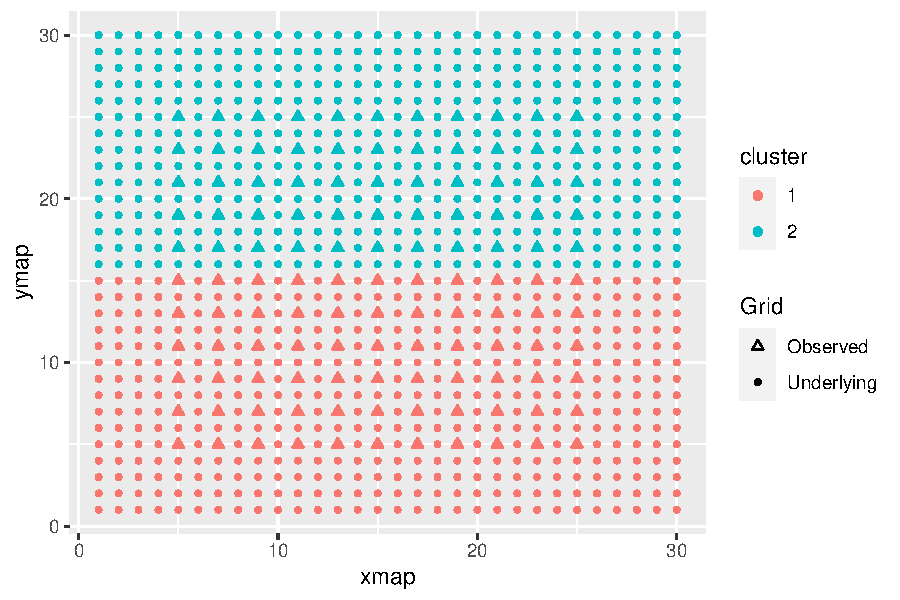
\includegraphics[width=\linewidth,]{spatio-temporal-model-arctic-sea-ice_files/figure-latex/grids-combined-1} 

}

\caption[Simulation Grids]{Underlying Process Grid and Observed Grid together, where the true cluster is also given.}\label{fig:grids-combined}
\end{figure}

\begin{figure}[tbp]

{\centering 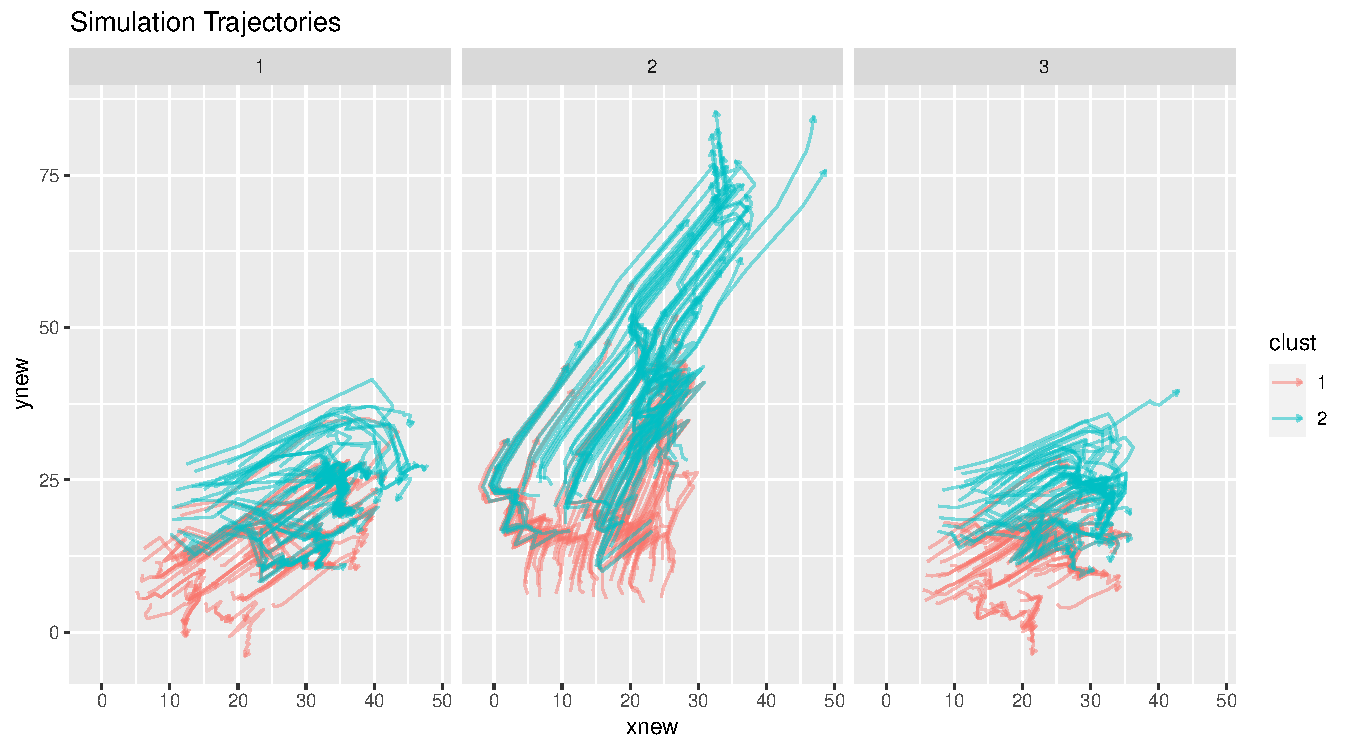
\includegraphics[width=\linewidth,]{spatio-temporal-model-arctic-sea-ice_files/figure-latex/traj-wrap-1} 

}

\caption{Trajectory Plots for each Simulated Data Set }\label{fig:traj-wrap}
\end{figure}

\begin{table}

\caption{\label{tab:parms-table}Parameters Y for Underlying Process for Each Cluster}
\centering
\begin{tabular}[t]{rrrrrrrrrrr}
\toprule
\multicolumn{1}{c}{ } & \multicolumn{5}{c}{X} & \multicolumn{5}{c}{Y} \\
\cmidrule(l{3pt}r{3pt}){2-6} \cmidrule(l{3pt}r{3pt}){7-11}
Cluster & $\sigma^{2}_{x}$ & $\phi_{x,s}$ & $\tau_{x}$ & $Nugget_x$ & $\mu_x$ & $\sigma^{2}_{y}$ & $\phi_{y,s}$ & $\tau_{y}$ & $Nugget_y$ & $\mu_y$\\
\midrule
\addlinespace[0.3em]
\multicolumn{11}{l}{\textbf{Simulation 1}}\\
\hspace{1em}1 & 5 & 5 & 5 & 0 & 2.0 & 5 & 5 & 5 & 0 & 1.5\\
\hspace{1em}2 & 40 & 60 & 10 & 0 & 10.0 & 80 & 50 & 10 & 0 & 6.0\\
\addlinespace[0.3em]
\multicolumn{11}{l}{\textbf{Simulation 2}}\\
\hspace{1em}1 & 1 & 10 & 5 & 0 & 0.5 & 2 & 10 & 7 & 0 & 2.0\\
\hspace{1em}2 & 20 & 20 & 2 & 0 & 2.0 & 25 & 20 & 3 & 0 & 4.0\\
\addlinespace[0.3em]
\multicolumn{11}{l}{\textbf{Simulation 3}}\\
\hspace{1em}1 & 2 & 10 & 5 & 0 & 1.5 & 2 & 10 & 5 & 0 & 1.0\\
\hspace{1em}2 & 20 & 20 & 10 & 0 & 6.0 & 20 & 30 & 10 & 0 & 3.0\\
\bottomrule
\end{tabular}
\end{table}

\hypertarget{clustering-method}{%
\subsection{Clustering Method}\label{clustering-method}}

\begin{figure}[tbp]

{\centering 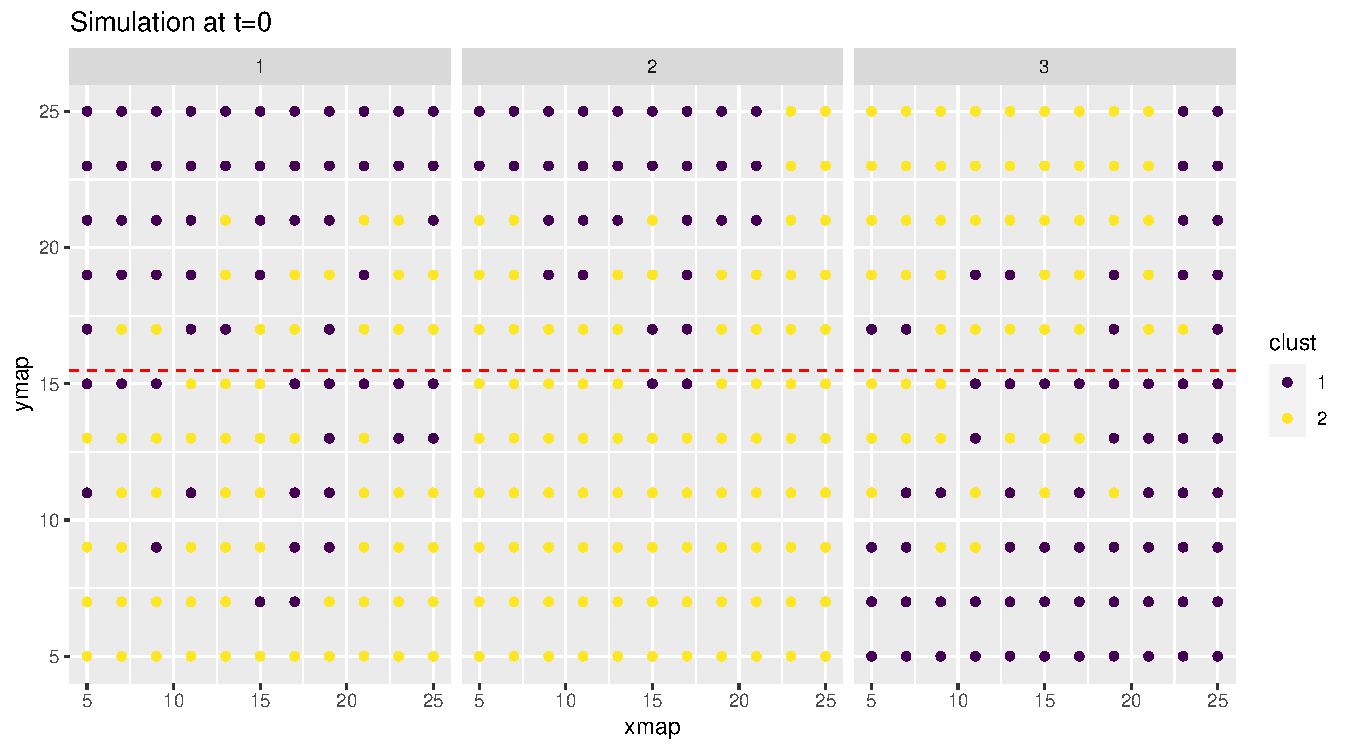
\includegraphics[width=\linewidth,]{spatio-temporal-model-arctic-sea-ice_files/figure-latex/plot-og-clus-1} 

}

\caption{Clusterings of Observed Data on Original Grid}\label{fig:plot-og-clus}
\end{figure}

\begin{figure}[tbp]

{\centering 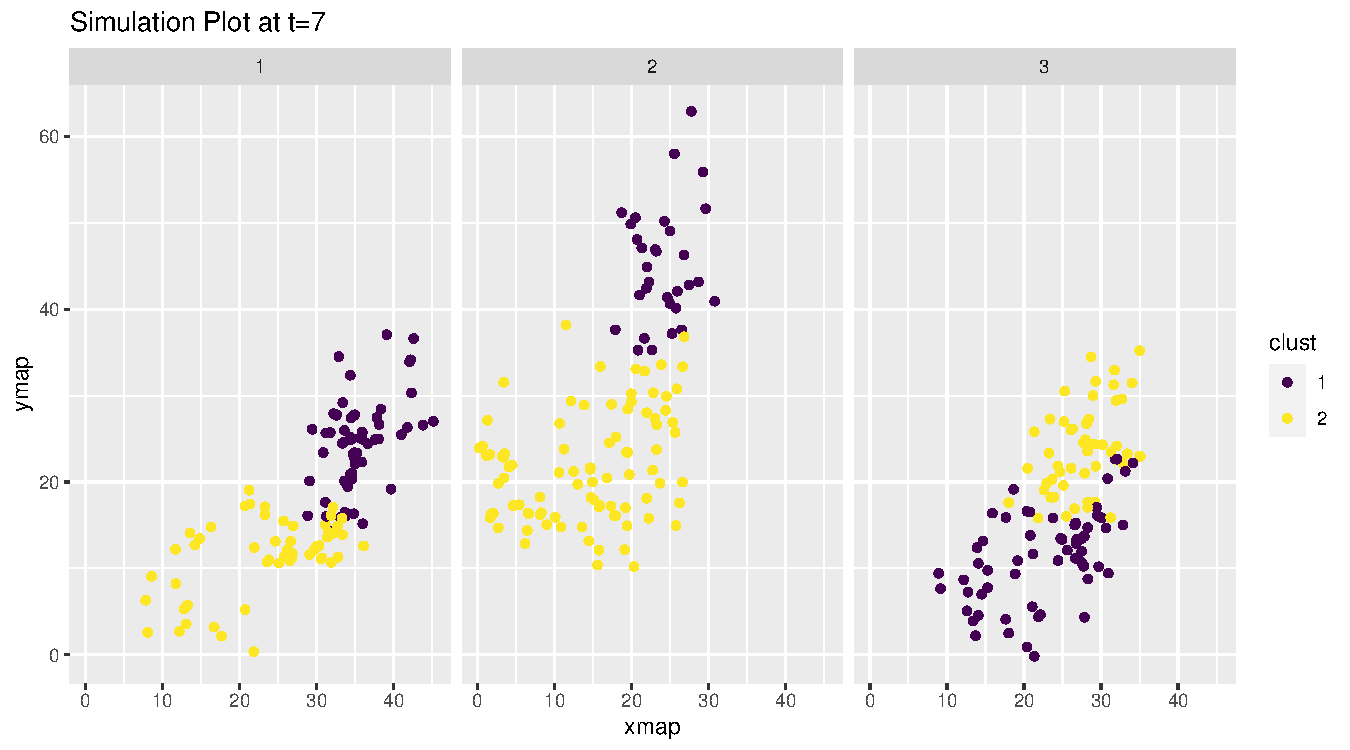
\includegraphics[width=\linewidth,]{spatio-temporal-model-arctic-sea-ice_files/figure-latex/all-clus-1} 

}

\caption{Clusterings of Observed Data on Final Day of Data Set}\label{fig:all-clus}
\end{figure}

Now our proposed spatio-temporal clustering method, using a bounding
box, is performed on each of the simulated datasets. Since the true
number of clusters is two, two is used as the \(k\) input in the k-means
clustering algorithm. The results are shown at two different time
points. First, the k-means determined clusters are plotted on the
initial grid to visualize how well our method performs when we can see
the true clusterings (see \cref{fig:plot-og-clus}). The cut-off for the
initially assigned cluster groupings is given by the red-dashed line. In
this figure, a majority of points seemed to be clustered correctly,
however, there are a number of misclassified points in each simulation.
In Simulation 1, most of the misclassifications happen along the border,
but seem to increase from left to right. Most of cluster 2 is clustered
correctly in Simulation 2, with the majority of the misclassification in
cluster 1 happening along the edges and boundary. Similarly, in
Simulation 3 most of the misclassifications are near the border, with a
handful along the right edge of cluster 2.

The clusters are also visualized on the last day of the week to see if
the clusters determined by the bounding box can distinguish movement
over time. In \cref{fig:all-clus}, there are distinguishable boundaries
between clusters for each of the simulations. Simulation 3 has a little
overlap along the boundary, but can still distinguish two continguous
clusters. Thus, by clustering using the movement features of a
trajectory, we are able to distinguish the different movement patterns
of the data with a clearly defined boundary. Some of the
misclassifications on the original grid may be due to the value of the
underlying process that was added to get the new location. This value
was determined by the closest grid cell of the underlying process by
Euclidean distance. If the point eventually becomes closer to the other
cluster, meaning that cluster's underlying process values are being
added to cause the movement, it will eventually start to move like it.
So, if it spends more time moving like cluster 1 than cluster 2, as an
example, it will most likely be classified as cluster 1, even if that
was not its initial cluster assignment.

\hypertarget{interpolation-method}{%
\subsection{Interpolation Method}\label{interpolation-method}}

\begin{table}

\caption{\label{tab:results-table}RMSE for Interpolation Methods}
\centering
\begin{tabular}[t]{rrrrrrrr}
\toprule
\multicolumn{2}{c}{Intersection} & \multicolumn{2}{c}{Linear} & \multicolumn{2}{c}{No Intersection} & \multicolumn{2}{c}{Bivariate} \\
\cmidrule(l{3pt}r{3pt}){1-2} \cmidrule(l{3pt}r{3pt}){3-4} \cmidrule(l{3pt}r{3pt}){5-6} \cmidrule(l{3pt}r{3pt}){7-8}
$X$ & $Y_{int}$ & $X$ & $Y_{lin}$ & $X_{no int}$ & $Y_{no int}$ & $X_{bi}$ & $Y_{bi}$\\
\midrule
\addlinespace[0.3em]
\multicolumn{8}{l}{\textbf{Simulation 1}}\\
\hspace{1em}1.50 & 1.51 & 1.04 & 1.23 & 1.43 & 1.29 & 1.54 & 1.67\\
\addlinespace[0.3em]
\multicolumn{8}{l}{\textbf{Simulation 2}}\\
\hspace{1em}1.54 & 1.55 & 1.45 & 1.54 & 1.47 & 1.49 & 1.63 & 1.58\\
\addlinespace[0.3em]
\multicolumn{8}{l}{\textbf{Simulation 3}}\\
\hspace{1em}1.41 & 1.40 & 0.95 & 0.92 & 1.46 & 1.51 & 1.43 & 1.51\\
\bottomrule
\end{tabular}
\end{table}

The same simulated data are also used to check the performance of our
spatio-temporal interpolation model. For each of the simulations,
another week of data is similarly simulated and clustered. Polygons for
each cluster are created and then the intersection polygons for each
weeks clusters are found. Once again, intersections represent the
spatio-temporal neighbors of the data within that intersection. Next,
10\% of the data for the first week are randomly assigned to be missing.
Then univariate models for each coordinate are developed to obtain our
estimates of the missing locations.

In order to have a baseline method for comparison, we also used linear
interpolation on the same data. Linear interpolation estimates an
objects unknown location along a straight-line path between two known
locations. It has been shown to work well for trajectories that follow a
straight-line path and sampled at a high rate. On the other hand, it
tends to underperform when a trajectory follows a curved path or is not
heavily sampled \citep{wentz_comparison_2003, guo_improved_2011}.
Another method used for comparison is similar to our proposed method,
except now the intersections are ignored. Instead a model was developed
using all known points for \(t-1\), \(t\), and \(t+1\) (this essentially
ignores the non-stationarity aspect of our data). The Root Mean Square
Error (RMSE) for each simulation and interpolation method can be found
in \cref{tab:results-table}.

Our interpolation method never seems to outperform linear interpolation.
Further, only in Simulation 3 does running the model within each
intersection perform better than the overall model. However, since each
cluster was created with different movements,
\cref{tab:results-table-by-clust} breaks out the RMSE calculations by
cluster to see if there are different areas where our proposed method
may perform better. If just strictly comparing our proposed method to
linear interpolation for now, linear interpolation performs better in
Simulation 1 and Simulation 3. In Simulation 2, our method outperforms
linear interpolation for \(y\) in cluster 2. For Simulation 2 in
\cref{fig:traj-plot}, the \(y\)-values of cluster 2 are more spread out
and curved than the others. The other simulations may have some
curvature, but samples are taken closer together, or the data may be
spread out but mostly linear. Nonetheless, the performance of linear
interpolation is not surprising as there are long periods of linear
movement in each of the simulations, so the results may be dependent on
what points were randomly removed. Additionally, linear interpolation
can not estimate the first or last point of a trajectory, so there are
fewer predicted locations used to calculate the RMSE. Thus, these
simulations show that linear interpolation generally outperforms our
method, but our methods shows promise with curved data that may not be
highly sampled.

The results regarding intersection creation are mixed, with creating
intersections only being beneficial for Simulation 3. However, these
results may be impacted by some of the intersections not containing
muhch data, which may impact model development. Through the simulations
we also found that having a fine enought grid for the initial starting
values in the prediction function is key. If the grid is too coarse,
this can impact the accuracy of the estimations.

\begin{table}

\caption{\label{tab:results-table-by-clust}RMSE for Interpolation Methods by cluster}
\centering
\begin{tabular}[t]{rrrrrrrrr}
\toprule
\multicolumn{1}{c}{ } & \multicolumn{2}{c}{Intersection} & \multicolumn{2}{c}{Linear} & \multicolumn{2}{c}{No Intersection} & \multicolumn{2}{c}{Bivariate} \\
\cmidrule(l{3pt}r{3pt}){2-3} \cmidrule(l{3pt}r{3pt}){4-5} \cmidrule(l{3pt}r{3pt}){6-7} \cmidrule(l{3pt}r{3pt}){8-9}
Cluster & $X_{int}$ & $Y_{int}$ & $X_{lin}$ & $Y_{lin}$ & $X_{no int}$ & $Y_{no int}$ & $X_{bi}$ & $Y_{bi}$\\
\midrule
\addlinespace[0.3em]
\multicolumn{9}{l}{\textbf{Simulation 1}}\\
\hspace{1em}1 & 1.41 & 1.58 & 0.82 & 1.16 & 1.54 & 1.28 & 1.41 & 1.77\\
\hspace{1em}2 & 1.57 & 1.47 & 1.19 & 1.27 & 1.35 & 1.29 & 1.63 & 1.59\\
\addlinespace[0.3em]
\multicolumn{9}{l}{\textbf{Simulation 2}}\\
\hspace{1em}1 & 1.70 & 1.64 & 1.32 & 1.33 & 1.66 & 1.60 & 1.80 & 1.72\\
\hspace{1em}2 & 1.50 & 1.52 & 1.50 & 1.61 & 1.40 & 1.45 & 1.57 & 1.54\\
\addlinespace[0.3em]
\multicolumn{9}{l}{\textbf{Simulation 3}}\\
\hspace{1em}1 & 1.46 & 1.48 & 1.16 & 1.10 & 1.43 & 1.44 & 1.49 & 1.51\\
\hspace{1em}2 & 1.35 & 1.31 & 0.65 & 0.67 & 1.49 & 1.58 & 1.36 & 1.51\\
\bottomrule
\end{tabular}
\end{table}

\begin{table}

\caption{\label{tab:cp-table-sim}Proportion of Prediction interval containing observed and Average Standard Deviation of Estimates for Simulated Data}
\centering
\begin{tabular}[t]{lrrrr}
\toprule
Method & \$Coverage\_\{X\}\$ & Avg S\$D\_\{X\}\$ & \$Coverage\_\{Y\}\$ & Avg S\$D\_\{Y\}\$\\
\midrule
\addlinespace[0.3em]
\multicolumn{5}{l}{\textbf{Simulation 1}}\\
\hspace{1em}Univariate & 0.2571429 & 0.3832179 & 0.2714286 & 0.3506978\\
\hspace{1em}Bivariate & 0.0142857 & 0.0162862 & 0.0142857 & 0.0351810\\
\addlinespace[0.3em]
\multicolumn{5}{l}{\textbf{Simulation 2}}\\
\hspace{1em}Univariate & 0.2142857 & 0.3486122 & 0.1964286 & 0.3784616\\
\hspace{1em}Bivariate & 0.0000000 & 0.0012624 & 0.0000000 & 0.0012609\\
\addlinespace[0.3em]
\multicolumn{5}{l}{\textbf{Simulation 3}}\\
\hspace{1em}Univariate & 0.2432432 & 0.3189445 & 0.3108108 & 0.3365939\\
\hspace{1em}Bivariate & 0.0135135 & 0.0010500 & 0.0000000 & 0.0010501\\
\bottomrule
\end{tabular}
\end{table}

A benefit of using a model-based approach to interpolate missing
locations is that we are able to determine the uncertainty of the
estimate. To do so, conditional draws of the unobserved values given the
observed values are used to quantify the uncertainty. This is
accomplished by exploiting an advantage of Vecchia's Approximation that
approximate draws from a Gaussian Process model can be made through the
inverse Cholesky Factor \citep{guinness_permutation_2018}. Therefore,
for each model, 30 simulations of predictions are conducted to calculate
the standard deviation. These can then be used to create an interval of
our estimates. The intervals are found by \(\hat{x} \pm (2*sd_x)\) and
\(\hat{y} \pm (2*sd_y)\), where \(\hat{x}\) and \(\hat{y}\) are the
predictions, and \(sd_x\) and \(sd_y\) are the standard deviations
determined by the conditional simulations. Next, we found the proportion
of the intervals that contain the true value, otherwise known as
coverage. For each simulation the coverage can be found in
\cref{tab:cp-table-sim} along with the average standard deviation values
to show typical interval width. The proportions in this table are low,
mainly in the 20\%-30\% range. Like the RMSE values, the proportions can
be separated by cluster, which are found in \cref{tab:cp-sim-table}.
These values are also low, with no proportion over 50\%. Also, the
\(x\)-values in cluster 1 for Simulation 3 have almost no intervals that
contain the true value. The standard deviation vlaues in
\cref{tab:cp-table-sim} are also low, meaning there is not much
variability among the predictions and the intervals are narrow. The low
coverage values show that the model has room for improvement in terms of
prediction accuracy.

\hypertarget{results}{%
\section{Results}\label{results}}

\begin{figure}[tbp]

{\centering 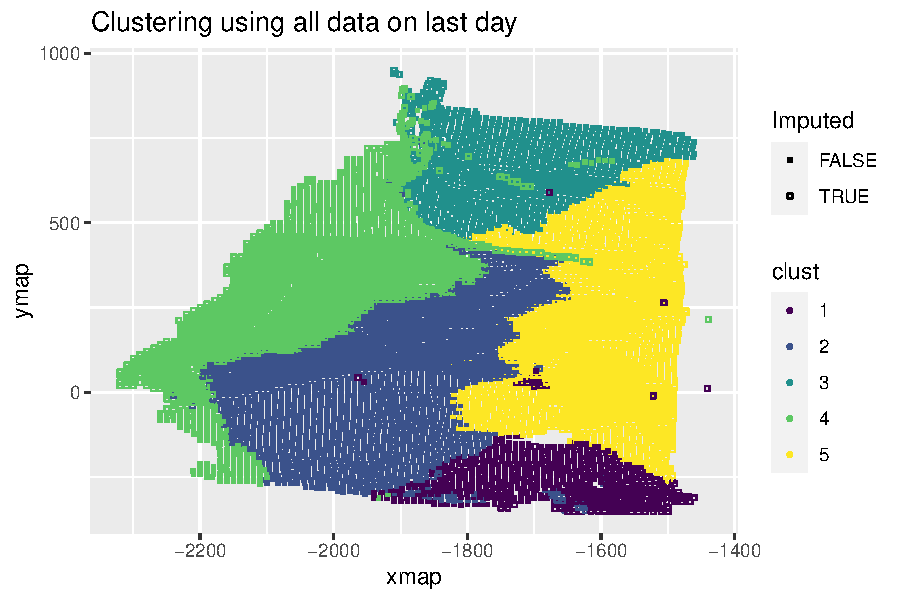
\includegraphics[width=\linewidth,]{spatio-temporal-model-arctic-sea-ice_files/figure-latex/ex-result-1} 

}

\caption{Results of Clustering using Bounding Box Method for all the Data}\label{fig:ex-result}
\end{figure}

\begin{figure}[tbp]

{\centering 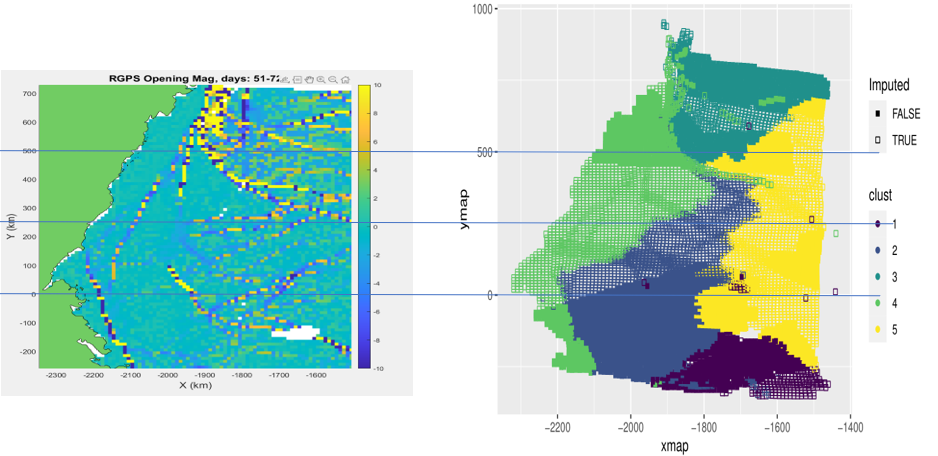
\includegraphics[width=1\linewidth,]{images/all_weeks_comp_correct} 

}

\caption{Comparison of our method to results of a previous method, which find cracks using a kinematic algorithm}\label{fig:all-week-comp}
\end{figure}

The simulation results showed some promise for our methods, so next the
methods are applied on the ice motion dataset.

\hypertarget{clustering-using-all-data}{%
\subsection{Clustering Using All Data}\label{clustering-using-all-data}}

First, we used our spatio-temporal clustering method by creating
bounding boxes around each \(g_j\). Once the bounding box features were
calculated and standardized, the number of clusters were determined
using the silhouette statistic. The silhouette statistic for the full
trajectory data suggested five clusters. The results from the clustering
algorithm are shown in \cref{fig:ex-result}. In \cref{fig:ex-result}
each of the colors represent one cluster; each of the squares represent
the last location in the dataset for each \(g_j\). The unfilled squares
represent missing data at this time, where the square location is
determined by it's last known location. We hypothesize that cracks in
the sea ice will be found along the boundaries of the clusters. In the
middle of some clusters, there are some singular points whose cluster
membership does not match its neighbors. In practicality these point
will belong to the cluster as its neighbors and a crack is not
considered to have formed here. In the future, a post-processing filter
to address these anomalies can be developed.

To see how well our method is performing, we can compare it to other sea
ice crack detection methods. One such method plots the deformation data
using a kinematic crack algorithm using the RGPS data
\citep{peterson_evaluating_2011}. \cref{fig:all-week-comp} gives a
comparison of our bounding box clustering method and the kinematic crack
algorithm using side-by-side plots. It is important to note that the
plot of the deformation data does not represent the true ice cracks,
just the cracks determined by this method. The plots are aligned so that
their axes match up for easier comparison. The lines given in the left
figure are derived from the opening magnitude of the ice sheet. Most of
the figure has a color around zero, denoting no opening, whereas
potential cracks are found with the dark blue or yellow. Many of our
cluster boundaries match up with the cracks identified by the kinematic
crack algorithm, though our proposed method is limited by the number of
clusters. For example, on the bottom left of both pltos, there is a line
that goes down and to the right. At the bottom right of both plots,
there is a line through the hole in the points. Additionally, towards
the top of both plots, there is a curved boundary that starts at the top
of the ice sheet and moves to the bottom left in a curved manner.

\hypertarget{clusterings-by-weeks}{%
\subsection{Clusterings By Weeks}\label{clusterings-by-weeks}}

Since trajectories can be long, it is also useful to look at
sub-trajectories as we lose information be clustering the whole
trajectory, which impacts results. Through some testing of our methods,
we found that by week was the smallest time period we could successfully
cluster, as anything smaller led to large changes in the clusterings
between each week (unstable). We would expect the weeks to have
different clusters, but would also expect there to be some continuity
between them. The clusters by week can be found in
\cref{fig:by-week-cluster-plot}, where can see some similarities in
clusters over time. In the clusters for week 1 and week 2, there is a
line moving from the top and down to the left, which is seen in the
kinematic crack algorithm, but not in \cref{fig:ex-resutls}. This is an
example of where clustering the sub-trajectories may provide additional
information.

Additionally, we had a picture from Day 66 of our dataset, which gives
an image of recurring leads based on visible and AVHRR data
\citep{eicken_sea_2015}. This would correspond to our week 3 cluster
plot. \cref{fig:week-comp} includes grid lines to aid in the comparison
of the pictures, due to the aspect ratios not aligning perfectly. One
major crack stands out in both images. Our boundary between cluster 1
and 3 aligns until about (-1880, 400), at this point our boundary curves
in more steeply. Eventually, the upper section of the cluster boundary
between cluster 5 and 6 continue the crack.

\begin{figure}[tbp]

{\centering \includegraphics[width=\linewidth,]{spatio-temporal-model-arctic-sea-ice_files/figure-latex/by-week-cluster-plot-1} 

}

\caption{Results of Clustering using Bounding Box Method by Week}\label{fig:by-week-cluster-plot}
\end{figure}

\begin{figure}[tbp]

{\centering 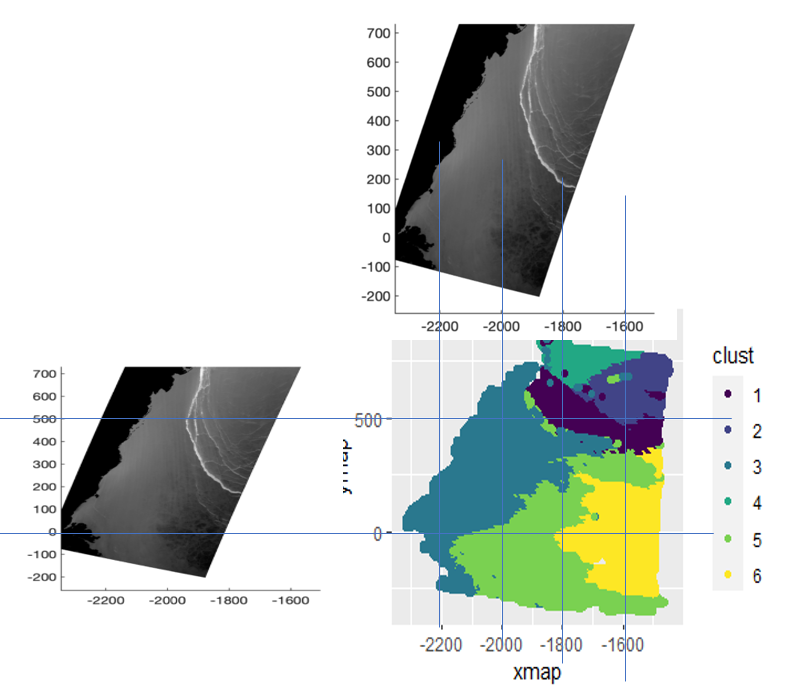
\includegraphics[width=0.8\linewidth,]{images/week-comp} 

}

\caption{Comparison of our method to results of a previous method for Week 3}\label{fig:week-comp}
\end{figure}

\hypertarget{univariate-interpolation-1}{%
\subsection{Univariate Interpolation}\label{univariate-interpolation-1}}

\begin{figure}[tbp]

{\centering 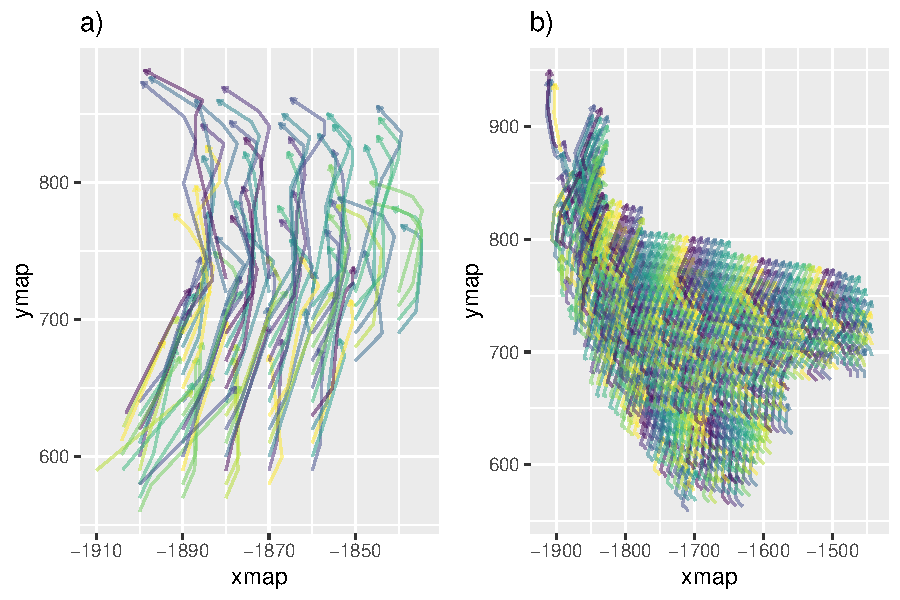
\includegraphics[width=\linewidth,]{spatio-temporal-model-arctic-sea-ice_files/figure-latex/int-best-plots-1} 

}

\caption{Trajectories for a) Week 2 Cluster 1, where our method peforms best and b) Week 2 Cluster 5, where linear interpolation performs best. These are instances where our method outperforms linear interpolation}\label{fig:int-best-plots}
\end{figure}

\begin{table}

\caption{\label{tab:results-table2}RMSE for Interpolation Methods}
\centering
\begin{tabular}[t]{rrrrrrrr}
\toprule
\multicolumn{2}{c}{Intersection} & \multicolumn{2}{c}{Linear} & \multicolumn{2}{c}{No Intersection} & \multicolumn{2}{c}{Bivariate} \\
\cmidrule(l{3pt}r{3pt}){1-2} \cmidrule(l{3pt}r{3pt}){3-4} \cmidrule(l{3pt}r{3pt}){5-6} \cmidrule(l{3pt}r{3pt}){7-8}
$X_{int}$ & $Y_{int}$ & $X_{lin}$ & $Y_{lin}$ & $X_{noint}$ & $Y_{noint}$ & $X_{bi}$ & $Y_{bi}$\\
\midrule
\addlinespace[0.3em]
\multicolumn{8}{l}{\textbf{Week 1}}\\
\hspace{1em}3.25 & 3.21 & 1.53 & 4.18 & 3.09 & 2.88 & 3.17 & 7.72\\
\addlinespace[0.3em]
\multicolumn{8}{l}{\textbf{Week 2}}\\
\hspace{1em}3.14 & 3.06 & 2.00 & 1.40 & 3.20 & 3.15 & 3.19 & 3.11\\
\addlinespace[0.3em]
\multicolumn{8}{l}{\textbf{Week 3}}\\
\hspace{1em}3.17 & 3.09 & 1.03 & 1.21 & 3.19 & 3.15 & 3.13 & 3.04\\
\bottomrule
\end{tabular}
\end{table}

Next, we tested our spatio-temporal interpolation method on the ice
motion dataset in order to see how it performs on real data. We did not
estimate the already missing data for validation purposes.For cross
validation, we can create a model for an intersection and time. The
intersections were found using the clusters in
\cref{fig:by-week-cluster-plot}. In each intersection and time
combination, 10\% of the known data was removed from the dataset. Next,
we found all the observed data in that intersection for \(t-1\), \(t\),
and \(t+1\) to obtain the spatio-temporal neighbors. Then, using the
observed data, the model was fit and used to estimate the points
assigned to be missing. This was done for all intersection and time
combinations for the three weeks. The RMSE for each week can be found in
\cref{tab:results-table2}. Additionally, linear interpolation and the
overall model method was performed on the same missing data for
comparison, similar to the simulated data. However, since linear
interpolation is unable to estimate data without a point before and
after (essentially the beginning or end of the week), it is not exactly
a one-to-one comparison. Also, for the overall model, due to the
log-likelihood failing to converge, a model was only able to be
developed for one day in week 1. Hence, the week 1 RMSE value for this
week is not useful for comparison. In \cref{tab:results-table2}, linear
interpolation outperforms the other methods except for the \(y\)-values
in week 1.

However, when looking at the trajectory plot in \cref{traj-plot}, some
of the trajectories in the plot are more linear than others (ie. have
different movements defined by the clusters). Based on our simulation
study, our method may have improvement over linear interpolation on
curved data and less-sampled trajectories. Thus, the RMSE values are
also broken out by cluster, as these are the groups of movement patterns
in the data. These values can be found for each week in
\cref{tab:results-clust1-actual}, \cref{tab:results-clust2-actual}, and
\cref{tab:results-clust3-actual}. Once again, linear interpolation
generally outperforms our method, but there are two exceptions. For week
1 and week 2, linear interpolation performed the worst of the other two
methods for cluster 1. In \cref{fig:by-week-cluster-plot}, cluster 1 for
both of these weeks is at the top of the plot. When comparing this
cluster location to the trajectory plot in \cref{fig:traj-plot}, the top
of the figure is where the most curved movement happens with a longer
distance traveled over time. Hence, linear interpolation may not work as
well here. Further, \cref{fig:int-best-plot} zooms in on an example for
week 2 where our intersection method performs best (plot (a)) and linear
interpolation performs best (plot (b)). \cref{fig:int-best-plot}a) is
cluster 1, where the observed points are more spread out along the
trajectory. On the other hand \cref{fig:int-best-plot}b) has small,
linear movement, which is why linear interpolation performs best.

As previously stated, though the RMSE for the overall model was lower
than the intersection model in week 1, this only represents one day's
worth of data. So, for cluster 1 in week 2, there were mixed results
between the two model methods as one performs better for \(x\) and the
other for \(y\). Overall, when comparing the two model-based approaches,
we find mixed results when comparing their performance, but the
intersection model performs better more often. Once again, these results
show that our method has some promise with non-linear and less-sampled
data.

\begin{table}

\caption{\label{tab:results-clust1-actual}RMSE by Cluster for Week 1 for Interpolation Methods}
\centering
\begin{tabular}[t]{rrrrrrrrr}
\toprule
\multicolumn{1}{c}{ } & \multicolumn{2}{c}{Intersection} & \multicolumn{2}{c}{Linear} & \multicolumn{2}{c}{No Intersection} & \multicolumn{2}{c}{Bivariate} \\
\cmidrule(l{3pt}r{3pt}){2-3} \cmidrule(l{3pt}r{3pt}){4-5} \cmidrule(l{3pt}r{3pt}){6-7} \cmidrule(l{3pt}r{3pt}){8-9}
Cluster & $X_{int}$ & $Y_{int}$ & $X_{lin}$ & $Y_{lin}$ & $X_{noint}$ & $Y_{noint}$ & $X_b$ & $Y_b$\\
\midrule
1 & 3.07 & 4.10 & 3.20 & 13.04 & 2.52 & 3.61 & 3.16 & 17.68\\
2 & 4.36 & 4.30 & 0.19 & 0.36 & 4.26 & 3.98 & 4.58 & 4.63\\
3 & 3.08 & 3.10 & 1.31 & 3.07 & 2.17 & 2.72 & 2.85 & 9.88\\
4 & 3.10 & 2.85 & 1.40 & 2.44 & 2.46 & 2.34 & 2.97 & 2.79\\
5 & 3.91 & 3.67 & 0.77 & 3.17 & 3.89 & 2.55 & 3.99 & 8.78\\
\addlinespace
6 & 3.10 & 3.06 & 1.89 & 5.64 & 2.63 & 3.35 & 3.23 & 4.69\\
\bottomrule
\end{tabular}
\end{table}

\begin{table}

\caption{\label{tab:results-clust2-actual}RMSE by Cluster for Week 2 for Interpolation Methods}
\centering
\begin{tabular}[t]{rrrrrrrrr}
\toprule
\multicolumn{1}{c}{ } & \multicolumn{2}{c}{Intersection} & \multicolumn{2}{c}{Linear} & \multicolumn{2}{c}{No Intersection} & \multicolumn{2}{c}{Bivariate} \\
\cmidrule(l{3pt}r{3pt}){2-3} \cmidrule(l{3pt}r{3pt}){4-5} \cmidrule(l{3pt}r{3pt}){6-7} \cmidrule(l{3pt}r{3pt}){8-9}
Cluster & $X_{int}$ & $Y_{int}$ & $X_{lin}$ & $Y_{lin}$ & $X_{noint}$ & $Y_{noint}$ & $X_b$ & $Y_b$\\
\midrule
1 & 3.00 & 2.93 & 3.24 & 3.32 & 2.62 & 3.04 & 3.05 & 4.60\\
2 & 2.94 & 2.89 & 2.55 & 1.03 & 2.89 & 2.94 & 3.04 & 2.88\\
3 & 2.94 & 2.90 & 1.58 & 1.99 & 2.95 & 3.03 & 2.95 & 2.91\\
4 & 3.26 & 3.13 & 1.40 & 0.52 & 3.45 & 3.19 & 3.37 & 3.17\\
5 & 4.23 & 4.16 & 0.31 & 0.37 & 4.41 & 4.20 & 4.32 & 4.28\\
\bottomrule
\end{tabular}
\end{table}

\begin{table}

\caption{\label{tab:results-clust3-actual}RMSE by Cluster for Week 3 for Interpolation Methods}
\centering
\begin{tabular}[t]{rrrrrrrrr}
\toprule
\multicolumn{1}{c}{ } & \multicolumn{2}{c}{Intersection} & \multicolumn{2}{c}{Linear} & \multicolumn{2}{c}{No Intersection} & \multicolumn{2}{c}{Bivariate} \\
\cmidrule(l{3pt}r{3pt}){2-3} \cmidrule(l{3pt}r{3pt}){4-5} \cmidrule(l{3pt}r{3pt}){6-7} \cmidrule(l{3pt}r{3pt}){8-9}
Cluster & $X_{int}$ & $Y_{int}$ & $X_{lin}$ & $Y_{lin}$ & $X_{noint}$ & $Y_{noint}$ & $X_b$ & $Y_b$\\
\midrule
1 & 2.85 & 2.85 & 2.04 & 2.67 & 2.70 & 3.04 & 2.94 & 2.84\\
2 & 2.81 & 2.95 & 2.15 & 2.06 & 2.65 & 2.85 & 2.68 & 2.97\\
3 & 3.65 & 3.59 & 0.19 & 0.44 & 3.75 & 3.60 & 3.70 & 3.61\\
4 & 2.67 & 2.78 & 1.53 & 0.72 & 2.87 & 2.92 & 2.61 & 2.87\\
5 & 3.16 & 3.04 & 0.21 & 0.48 & 3.08 & 3.09 & 3.11 & 2.99\\
\addlinespace
6 & 3.21 & 3.01 & 0.28 & 0.55 & 3.23 & 3.01 & 3.25 & 3.03\\
\bottomrule
\end{tabular}
\end{table}

The proportion of the prediction intervals containing the observed data,
along with the average standard deviations are given in
\cref{tab:cp-table}. These values were found in the same way as the
simulated data. The standard deviations are higher than what was seen
with the simulated data, but the coverage is similar (ranging from
25\%-31\%). Once again, this can be broken down by cluster in
\cref{tab:cp-clust-actual}. However, once again, none of the values are
as large as desired. Through cluster 1 in week 1 has a coverage of over
50\% for \(x\). The model then may need further investigation and
development to increase this.

\begin{table}

\caption{\label{tab:cp-table}Proportion of Prediction interval containing observed and Average Standard Deviation for Ice Data}
\centering
\begin{tabular}[t]{lrrrr}
\toprule
Method & Proportion of X & Avg SD of X & Proportion of Y & Avg SD of Y\\
\midrule
\addlinespace[0.3em]
\multicolumn{5}{l}{\textbf{Week 1}}\\
\hspace{1em}Univariate & 0.2556491 & 0.7878753 & 0.2927257 & 0.8338038\\
\hspace{1em}Bivariate & 0.0054730 & 0.0157526 & 0.0179828 & 0.0874537\\
\addlinespace[0.3em]
\multicolumn{5}{l}{\textbf{Week 2}}\\
\hspace{1em}Univariate & 0.2630683 & 0.7509988 & 0.2980793 & 0.8104493\\
\hspace{1em}Bivariate & 0.0089376 & 0.0264320 & 0.0148398 & 0.0261314\\
\addlinespace[0.3em]
\multicolumn{5}{l}{\textbf{Week 3}}\\
\hspace{1em}Univariate & 0.2463850 & 0.7600099 & 0.2630986 & 0.7960184\\
\hspace{1em}Bivariate & 0.0037925 & 0.0096209 & 0.0068510 & 0.0191015\\
\bottomrule
\end{tabular}
\end{table}

Next, instead of a random hold-out of all of the data, we took a random
hold-out of points along the cluster borders. We are interested in
points along the cluster border as those might be locations of irregular
movement. Boundaries in the code are defined as points where some of its
neighbors are from a different cluster. Otherwise the process remains
the same as before. \cref{tab:border-cv-rmse} contains the RMSE values
for our proposed method and linear interpolation. The model with all the
data (no intersection) is not used for comparison here as these models
produced an error with issues in convergence of the log-likelihood. When
we just look at the weeks overall, our proposed model only outperforms
linear interpolation in week 1 for \(y\)-values. Furthermore, this was
broken out by cluster in \cref{tab:border-clust}. This shows similar
results as the random hold-out, with our method outperforming linear
interpolation in cluster 1 for week 1 and 2. Additionally, in week 1,
our method performs best for \(y\)-values for all clusters expect for
cluster 2.

As in prior sections, 30 conditional simulations were performed to
calculate the uncertainty. Using the standard deviation found from these
simulations we calculated an interval. Then the coverage, or the
proportion of intervals that contain the true value are calculated
(\cref{tab:cp-table-border}). Once again, as in \cref{tab:cp-table},
these values are low, with most intervals not containing the true value.
In \cref{tab:cp-table-border-clust}, these values are broken out by
cluster. The values do seem slightly higher in the instances where our
method performs best.

\begin{table}

\caption{\label{tab:border-cv-rmse}RMSE for Interpolation Methods on Cluster Border Points}
\centering
\begin{tabular}[t]{rrrr}
\toprule
\multicolumn{2}{c}{Intersection} & \multicolumn{2}{c}{Linear} \\
\cmidrule(l{3pt}r{3pt}){1-2} \cmidrule(l{3pt}r{3pt}){3-4}
$X_{int}$ & $Y_{int}$ & $X_{lin}$ & $Y_{lin}$\\
\midrule
\addlinespace[0.3em]
\multicolumn{4}{l}{\textbf{Week 1}}\\
\hspace{1em}3.050927 & 3.252175 & 1.517341 & 4.147691\\
\addlinespace[0.3em]
\multicolumn{4}{l}{\textbf{Week 2}}\\
\hspace{1em}3.304622 & 3.265918 & 2.038981 & 1.832126\\
\addlinespace[0.3em]
\multicolumn{4}{l}{\textbf{Week 3}}\\
\hspace{1em}3.029221 & 2.954847 & 0.992153 & 1.240639\\
\bottomrule
\end{tabular}
\end{table}

\begin{table}

\caption{\label{tab:border-clust-tab}RMSE by Cluster for Cross Validation Along Cluster Borders}
\centering
\begin{tabular}[t]{rrrrrrrrrrrrr}
\toprule
\multicolumn{1}{c}{ } & \multicolumn{4}{c}{Week 1} & \multicolumn{4}{c}{Week 2} & \multicolumn{4}{c}{Week 3} \\
\cmidrule(l{3pt}r{3pt}){2-5} \cmidrule(l{3pt}r{3pt}){6-9} \cmidrule(l{3pt}r{3pt}){10-13}
Cluster & $X_{int}$ & $Y_{int}$ & $X_{lin}$ & $Y_{lin}$ & $X_{int}$ & $Y_{int}$ & $X_{lin}$ & $Y_{lin}$ & $X_{int}$ & $Y_{int}$ & $X_{lin}$ & $Y_{lin}$\\
\midrule
1 & 2.417 & 3.891 & 2.351 & 8.327 & 2.830 & 3.049 & 3.819 & 5.192 & 2.688 & 2.853 & 1.883 & 2.618\\
2 & 3.814 & 4.095 & 0.212 & 0.263 & 2.936 & 2.960 & 2.388 & 0.989 & 2.718 & 2.848 & 1.879 & 1.916\\
3 & 2.574 & 3.025 & 1.149 & 3.568 & 2.935 & 3.052 & 1.456 & 1.972 & 3.490 & 3.295 & 0.218 & 0.427\\
4 & 2.474 & 2.811 & 1.280 & 2.796 & 3.270 & 3.218 & 1.318 & 0.537 & 2.924 & 3.227 & 2.255 & 1.458\\
5 & 3.994 & 3.622 & 0.597 & 4.339 & 4.155 & 3.916 & 0.431 & 0.336 & 2.837 & 2.831 & 0.216 & 0.490\\
\addlinespace
6 & 3.021 & 3.218 & 1.990 & 4.945 & NA & NA & NA & NA & 3.193 & 2.923 & 0.303 & 0.561\\
\bottomrule
\end{tabular}
\end{table}

\begin{table}

\caption{\label{tab:cp-table-border}Proportion of Prediction interval containing observed and Average Standard Deviation for Ice Data}
\centering
\begin{tabular}[t]{lrrrr}
\toprule
Week & Proportion of X & Avg SD of X & Proportion of Y & Avg SD of Y\\
\midrule
1 & 0.320 & 0.942 & 0.344 & 1.069\\
2 & 0.267 & 0.808 & 0.267 & 0.871\\
3 & 0.277 & 0.775 & 0.283 & 0.785\\
\bottomrule
\end{tabular}
\end{table}

\begin{table}

\caption{\label{tab:cp-table-border-clust}Proportion of Prediction interval containing observed by Cluster for Cluster Border}
\centering
\begin{tabular}[t]{rrrllrr}
\toprule
\multicolumn{1}{c}{ } & \multicolumn{2}{c}{Week 1} & \multicolumn{2}{c}{Week 2} & \multicolumn{2}{c}{Week 3} \\
\cmidrule(l{3pt}r{3pt}){2-3} \cmidrule(l{3pt}r{3pt}){4-5} \cmidrule(l{3pt}r{3pt}){6-7}
Cluster & $X_{s1}$ & $Y_{s1}$ & $X_{s2}$ & $Y_{s2}$ & $X_{s3}$ & $Y_{s3}$\\
\midrule
1 & 0.592 & 0.592 & 0.467 & 0.413 & 0.422 & 0.357\\
2 & 0.270 & 0.288 & 0.28 & 0.278 & 0.471 & 0.418\\
3 & 0.347 & 0.312 & 0.337 & 0.351 & 0.184 & 0.245\\
4 & 0.482 & 0.301 & 0.26 & 0.251 & 0.491 & 0.309\\
5 & 0.157 & 0.300 & 0.149 & 0.163 & 0.283 & 0.264\\
\addlinespace
6 & 0.273 & 0.396 &  &  & 0.177 & 0.254\\
\bottomrule
\end{tabular}
\end{table}

\hypertarget{discussion}{%
\section{Discussion}\label{discussion}}

Our bounding box clustering method was developed to group trajectories
by their movement, and to compensate for missing data. This method was
shown, through simulations and actual data, that the boundaries of the
clusters determined by the trajectory movements provide a reasonable
estimation of the location of ice cracks. However, a major drawback is
that since we used k-means clustering, our method relies on a
pre-defined number of clusters, which is unknown. Furthermore, with
having a set number of clusters, there is a limit on how many cluster
boundaries, representing cracks, that can be identified. Thus, not all
possible cracks will be identified. Our method suggest that other
approaches to extend this method to identify higher higher resolution
cracks. Also, our method provides information about how the ice sheet is
moving, which may also be important when developing climate models.

Through our simulated and ice motion data, we have demonstrated some
situations where our interpolation method is beneficial. First, it takes
into account the non-stationarity of the data, which generally shows
slight improvement over using all the data to develop a model. Instances
where our proposed method under performs the overall model may be due to
lack of data to develop a better model at smaller intersections.
Secondly, it showed improvements over linear interpolation for curved
and low-sampled data. Eventually, our proposed method should be tested
against curved interpolation methods, like cubic splines, that handle
curved data better. Thirdly, our proposed method is able to estimate
missing locations on the first and last day of a dataset, which is
impossible with linear interpolation. Finally, since creating a model,
we are able to calculate an uncertainty measure with the predictions.
Despite these benefits, linear interpolation performs better in most
cases. So the additional information about movement does not provide any
benefit if that trajectories does not provide any benefit if the
trajectories are linear and we are only interested in location
estimation.

An drawback of our method for finding spatio-temporal neighbors is that
if an object is not located within an intersection, it is removed from
the data used to develop the models. Thus, we could be losing valuable
information for model development to obtain the estimates. Typically
this only happens to the \(g_j\) on the edges of the ice sheet.

When developing the models with the Vecchia Approximation, some other
issues arise. The first is that when the temporal range is exceptionally
large, especially in comparison with the spatial range, the model be fit
as the log-likelihood does not converge. Additionally, the estimated
covariance parameters do not make sense practically even when the model
can be successfully fit. This is because the parameter values are large,
though the variance and spatial range values are sometimes reasonable
for the simulated data. For example, the large temporal range means that
the data is not changing much over time, and there is a strong
dependence over multiple lifetime's worth of data, which is not
realistic. Using the simulated data as an example, the covariance
parameter estimates for one of the intersection on the third day were:
\(\sigma^2\) = 77.91, \(\phi\) = 458, \(\tau\) = 686,239.164, \(c_0\) =
0. In this scenario, the temporal range is quite large, which may be due
to only working with a small amount of data that is not moving much over
time. This is especially true when considering the ice motion data.
Potentially obtaining more practical covariance parameter estimates may
lead to better predictions and a higher coverage.

Another potential source for error when using a space-time covariance
function is that variation in time is needed. Otherwise, if there is
only observed data for one of the three days used to create the model,
the model cannot be developed. Finally, another issue, mainly seen in
the overall model for week 1 in \cref{tab:border-cv-rmse}, is the
location columns were sometimes considered too linearly dependent to
form a model. Though taking a random subset of the data generally
allowed the model to converge.

\hypertarget{conclusion}{%
\section{Conclusion}\label{conclusion}}

Sea ice plays a vital role in the Earth's energy balance, as when cracks
form in the ice, warm air from the ocean is released into the
atmosphere. In order to determine where these cracks may form using only
the movement of the ice sheet, a bounding box is created around each
tracked trajectory. The features of the bounding box are used as input
into k-means. Once each \(g_j\) is assigned a cluster, a plot of the
results is created where the cluster boundaries would be the location
where ice cracks may form. This method seemed to identify similar cracks
as other ice crack detection methods. Next, using the information from
spatio-temporal neighbors of the missing points, we created a model for
interpolation of the missing points. While linear interpolation
typically outperforms our method, it showed some promise with nonlinear
and low-sampled data.

In the future, more work needs to be done in the univariate model
development for the interpolation to facilitate convergence in a wider
range of situations. Next, we would eventually like to investigate a
bivariate interpolation model to estimate both \(x\) and \(y\) at the
same time. Finally, at the moment our method is a two step process: find
clusters and create model in each cluster. Eventually, we would like to
turn this into a one step process, potentially using voronoi
tessellations and a piecewise Gaussian Process.

\bibliographystyle{agsm}
\bibliography{bibliography.bib}


\end{document}
